\documentclass{article}
\usepackage{amsmath,amsfonts,amssymb}
\usepackage{graphicx}
% vertical whitespace instead of indentation of paragraphs
\usepackage{parskip}

\title{On Longitudinal Emittance}
\author{W.D. Klotz, wdklotz@alecli.com}

\begin{document}
\maketitle

\section{Overview}
The standard formula for an upright ellipse in phase-space $\Delta\phi\otimes w$ is:
\begin{equation}
\frac{\Delta\phi^{2}}{\Delta\phi_{0}^{2}}+\frac{w^{2}}{w_{0}^{2}}=1 \label{}
\end{equation}
with $ \Delta\phi = \phi - \phi_{s} $ and $ w \equiv \delta\gamma = \Delta W/mc^{2} $.
$ \phi_{s} $ being the synchronous phase, $ mc^{2} $ the rest energy, W the total energy and $ \gamma $ the Lorentz factor.
It has the emittance
\begin{equation}
\epsilon_{w} = |\Delta\phi_{0}w_{0}| \label{}
\end{equation}
and units [rad].
The ellipse intersetcs the $ \Delta\phi $-axis at $ \Delta\phi_{0} $ and the $ w $-axis at $ w_{0} $.
The intersection with the $w$-axis determines the $\beta$-function by the relation $\beta_{w} = \epsilon_{w}/w_{0}^{2}$. Its units are [$rad$].

Let's change to new coordinates, for instance the pair of canonical variables   $ z\otimes \Delta p/p $, as it is used internally in Trace 3D.
The transformation from old to new coordinates is:
$ z = -\kappa\Delta\phi =  -\frac{\beta \lambda} {2 \pi}  \Delta\phi $ and $ \Delta p/p = \tau w = \gamma/(\gamma^{2}-1) w = (\gamma \beta^{2})^{-1} w $.
This gives the modified ellipse equation:
\begin{equation}
\frac{z^{2}}{{(\kappa\Delta\phi_{0})}^{2}}+\frac{(\Delta p/p)^{2}}{{(\tau w_{0})^{2}}}=1 \label{}
\end{equation}
which has the transformed emittance 
\begin{equation}
\epsilon_{z} =  \kappa|\Delta\phi_{0}|*\tau |w_{0}| = \kappa\tau\epsilon_{w} = \frac{\beta \lambda} {2 \pi} \gamma/(\gamma^{2}-1) \epsilon_{w} = \frac{\lambda} {2 \pi \gamma \beta} \epsilon_{w}\label{},
\end{equation}
with units [$m\times rad$]. Again the $\beta$-function is given by 
\begin{equation}
\beta_{z}=\epsilon_{z}/(\Delta p/p)_{0}^{2}=\kappa\tau\epsilon_{w}/(\tau w_{0})^2=\kappa/\tau\times\beta_{w}=\frac{\beta \lambda}{2 \pi}\frac{\gamma^2-1}{\gamma}\beta_{w},
\end{equation}
with units [$m$].

For the $ \Delta\phi\otimes\Delta W $ phase space, because $ \Delta W = mc^{2} w $, we have $ \kappa = 1 $ and $ \tau = mc^{2} $.
So that 
\begin{equation}
\epsilon_{W} = mc^{2}\epsilon_{w}\quad [rad\times eV] \label{}
\end{equation}
\begin{equation}
\beta_{W} = 1/mc^{2}\beta_{w}\quad  [rad/eV] \label{}
\end{equation}

Finally for the $ \Delta z\otimes\Delta W $ phase space we get the emittance
\begin{equation}
\epsilon_{zW} = \frac{\beta \lambda} {2 \pi}mc^{2}\epsilon_{w}\quad  [m\times eV] \label{}
\end{equation}
\begin{equation}
\beta_{zW} = \frac{\beta \lambda} {2 \pi}\frac{1}{mc^{2}}\beta_{w}\quad  [m/eV] \label{}
\end{equation}

The ESS conceptual design report uses the $•z\otimes z'$ phase space, i.e. the emittance $ \epsilon_{zz'} $. Since $ \delta\gamma = w = \beta^{2}\gamma^{3} \delta\beta / \beta = \beta^{2}\gamma^{3} z' $ and 
$\Delta\phi  = \frac{2\pi}{\beta\lambda}z$ we have:
\begin{equation}
\epsilon_{zz'} = \frac{\lambda}{2\pi\beta\gamma^{3}}\epsilon_{w} \label{}
\end{equation}
with units [$m\times rad$].

Instead of longitudinal position some people use arrival time. For the $ \Delta t \otimes \Delta W $ phase space we use 
$\Delta t = -(\beta c)^{-1} z = (\beta c)^{-1} \frac{\beta\lambda}{2\pi} \Delta \phi$ and get
\begin{equation}
\epsilon_{tW} = \frac{\lambda} {2 \pi c} mc^{2}\epsilon_{w}\quad  [sec\times eV]\label{}
\end{equation}

\section{Full Treatment}
The ellipse in normal form:
\begin{equation}
\frac{x^{2}}{a^{2}}+\frac{y^{2}}{b^{2}}= 1 \label{}
\end{equation}
defines the emittance $\epsilon$ as:
\begin{equation}
\epsilon= |a*b| \label{}
\end{equation}
Changing scales of $x,y$ coordinates:
$x= x'/\kappa$ and $y=y'/\tau$ and inserting into normal form:
\begin{equation}
\frac{x'^{2}}{(a\kappa)^{2}}+\frac{y'^{2}}{(b\tau)^{2}} = 1 \label{}
\end{equation}
gives scaled emittance $\epsilon'$ 
\begin{equation}
\epsilon'= |(a \kappa)*(b\tau)| = \kappa \tau \epsilon \label{}
\end{equation}
Let $\beta_x = x_0^{2}/\epsilon$ then $\beta_x = (x'/\kappa)^{2} / (\epsilon'/\kappa\tau) = \frac{\tau}{\kappa} \beta_x'$, we get
\begin{equation}
\beta_x' = \frac{\kappa}{\tau} \beta_x \label{}
\end{equation}
In phase space $\Delta\phi$, $z$ and $\Delta t$ are usually used as abscissa and $w$, $\Delta W$, $\Delta p/p$ and $z'$ as ordinates.
We use $\kappa$ to connect abscissa and $\tau$ to connect different ordinates. Six different combinations of abscissa can be made and 11 combinations
for ordinates. Their corresponding $\kappa$- and $\tau$-values are assembled in the following tables. \\

\begin{tabular}{|c|c|c|c|}
\hline
\multicolumn{4}{|c|}{\textbf{$\kappa$-values}} \\
\hline
wanted$\downarrow$ in terms of$\rightarrow$ & $\Delta\phi$ [rad]          &$z$ [m]        &$\Delta t$ [sec]    \\
\hline
$\Delta\phi$ [rad]                          &1                            &$2\pi/\lambda$ &$2\pi\beta c/\beta\lambda$ \\
$z$ [m]                                     &$\beta\lambda/2\pi$          &1              &$\beta c$  \\
$\Delta t$ [sec]                            &$\beta\lambda/(2\pi\beta c)$ &$1/\beta c$    &1   \\
\hline
\end{tabular} \\ \\

\begin{tabular}{|c|c|c|c|c|}
\hline
\multicolumn{5}{|c|}{\textbf{$\tau$-values}} \\
\hline
wanted$\downarrow$ in terms of
$\rightarrow$                  &$\delta\gamma = w$              &$\Delta W$ [eV]              &$\Delta p/p$        &$z'$ [rad]    \\
\hline
$\delta\gamma = w$             &1                               &$1/(mc^2)$                   &$\gamma\beta^2$     &$\gamma(\gamma\beta)^2$ \\ 
$\Delta W$ [eV]                &$mc^2$                          &1                            &$mc^2\gamma\beta^2$ &$mc^2\gamma^3\beta^2$ \\
$\Delta p/p$                   &$(\gamma\beta^2)^{-1}$          &$(mc^2\gamma\beta^2)^{-1}$   &1                   &$\gamma^2$ \\
$z'$ [rad]                     &$\gamma^{-1}(\gamma\beta)^{-2}$ &$(mc^2\gamma^3\beta^2)^{-1}$ &$\gamma^{-2}$       &1  \\
\hline
\multicolumn{5}{|l|}{with $W = mc^2 (\gamma-1)$ as kinetic energy.} \\
\hline
\end{tabular} \\ \\

Example: Phase space $z\otimes\Delta W$ in terms of $\Delta\phi\otimes\delta\gamma$: $\kappa = \beta\lambda/2\pi$, $\tau = mc^2$.
\begin{equation}
\epsilon_{zW} = \kappa\tau\epsilon_w=(\beta\lambda/2\pi) mc^2\epsilon_w.
\end{equation}
\begin{equation}
\beta_{zW} = \frac{\kappa}{\tau}\beta_w=\frac{\beta\lambda/2\pi}{mc^2}\beta_w.
\end{equation}

More interesting details about emittance definitions, normalized and unnormalized, and their units can be found in the UserManual of the \emph{TraceWin} program.

\section{Twiss Parameter Values}
To simplify we assume the twiss parameter $ \alpha = 0 $. The twiss  parameter $ \gamma $ then reduces to $ 1/{\beta} $
and only two free parameters $ \epsilon $ and $ \beta $ remain to describe the ellipse in phase space completely.

For small aplitude longitudinal oscillations the separatrix intersects the w-axis at \(w_{0}\) and is is given by

%\begin{align}
%w_{0}&=\frac{\Delta W} {mc^{2}} = \Delta\phi_{0}\sqrt{qE_{0}LT\beta_{s}^{3}\gamma_{s}^{3}\lambda sin(-\phi_{s})/2\pi mc^{2}} \label{w0} 
%\end{align}
\begin{align}
w_{0}&=\frac{\Delta W} {mc^{2}} = \sqrt{2qE_{0}LT\beta_{s}^{3}\gamma_{s}^{3}\lambda \phi_{s}^2 \sin(-\phi_{s})/\pi mc^{2}} \label{w0} 
\end{align}

With $w_{0}$ and $\Delta\phi_{0}$ the maximal emittance on the separatrix is given.
\begin{equation}
\epsilon_{w} = w_{0} * \Delta\phi_{0} \label{w1}
\end{equation}

and from (\ref{w1}) we get finally $\gamma_{0} = \epsilon_{w}/\Delta\phi_{0}^{2}$ and $\beta_{0} = 1/\gamma_{0}$.

%\begin{equation}
%\gamma_{0} = \epsilon_{w}/\Delta\phi_{0}^{2} = \sqrt{qE_{0}LT\beta_{s}^{3}\gamma_{s}^{3}\lambda sin(-\phi_{s})/2\pi mc^{2}} \label{}\end{equation}

NOTE: the two twiss parameters $\gamma_{0}$ and $\beta_{0}$ are completely defined by the emittance $\epsilon_{w}$, the cavity field $E_{0}$, rf-phase $\phi_{s}$, rf-wavelength $\lambda$ and particle impuls $\thicksim\gamma\beta$.

\section{Appendix}
\subsection{SIMULAC Variables}
\begin{table}[h]
\caption{\textbf{Variable Names}}
\centering
\begin{tabular}{ c c c c c }
\hline\hline
$\epsilon_{w}$ = emitw   &$\Delta\phi$ = Dphi      &$\Delta\phi_{0}$ = Dphi0   &$w$ = w                    &$w_{0}$ = w0 \\
$\epsilon_{W}$ = emitW   &$\Delta z$ = z           &$\Delta W$ = DW            &$\Delta p/p$ = Dp2p        &$\Delta p/p_0$ = Dp2p0 \\
$\epsilon_{z}$ = emitz   &$\beta_{z}$ = betaz      &$\gamma_z$ = gammaz        &$\alpha_z$ = alphaz        &$\lambda$ = lamb \\
$Ez_{avg}$ = EzAvg       &$Ez_{peak}$ = EzPeak     &$\phi_{+}$ = phi\_1        &$\phi_{-}$ = phi\_2        &$\psi$ = psi \\
$\gamma$ = gamma         &$\gamma\beta$ = gb       &$\beta$ = beta             &$E_0T$ = E0T               & $E_0LT$ = E0LT \\
$mc^2$ = m0c2            &$mc^3$ = m0c3            &$\epsilon_{xi}$ = emitx\_i &$\epsilon_{yi}$ = emity\_i &$\epsilon_{zi}$ = emitz\_i \\
$\beta_{xi}$ = betax\_i  &$\beta_{yi}$ = betay\_i  &$\alpha_{xi}$ = alfax\_i   &$\alpha_{yi}$ = alfay\_i   &$\gamma_{xi}$ = gamax\_i \\  
$\gamma_{yi}$ = gamay\_i &$\omega$ = omg           &$\phi$ = phi               &$\phi_{s}$ = phisoll       &$\Delta W/W$  = DT2T \\
$W$ = Tkin
\end{tabular}
\end{table}

\subsection{Relations Between Ellipse and Twiss Parameters}
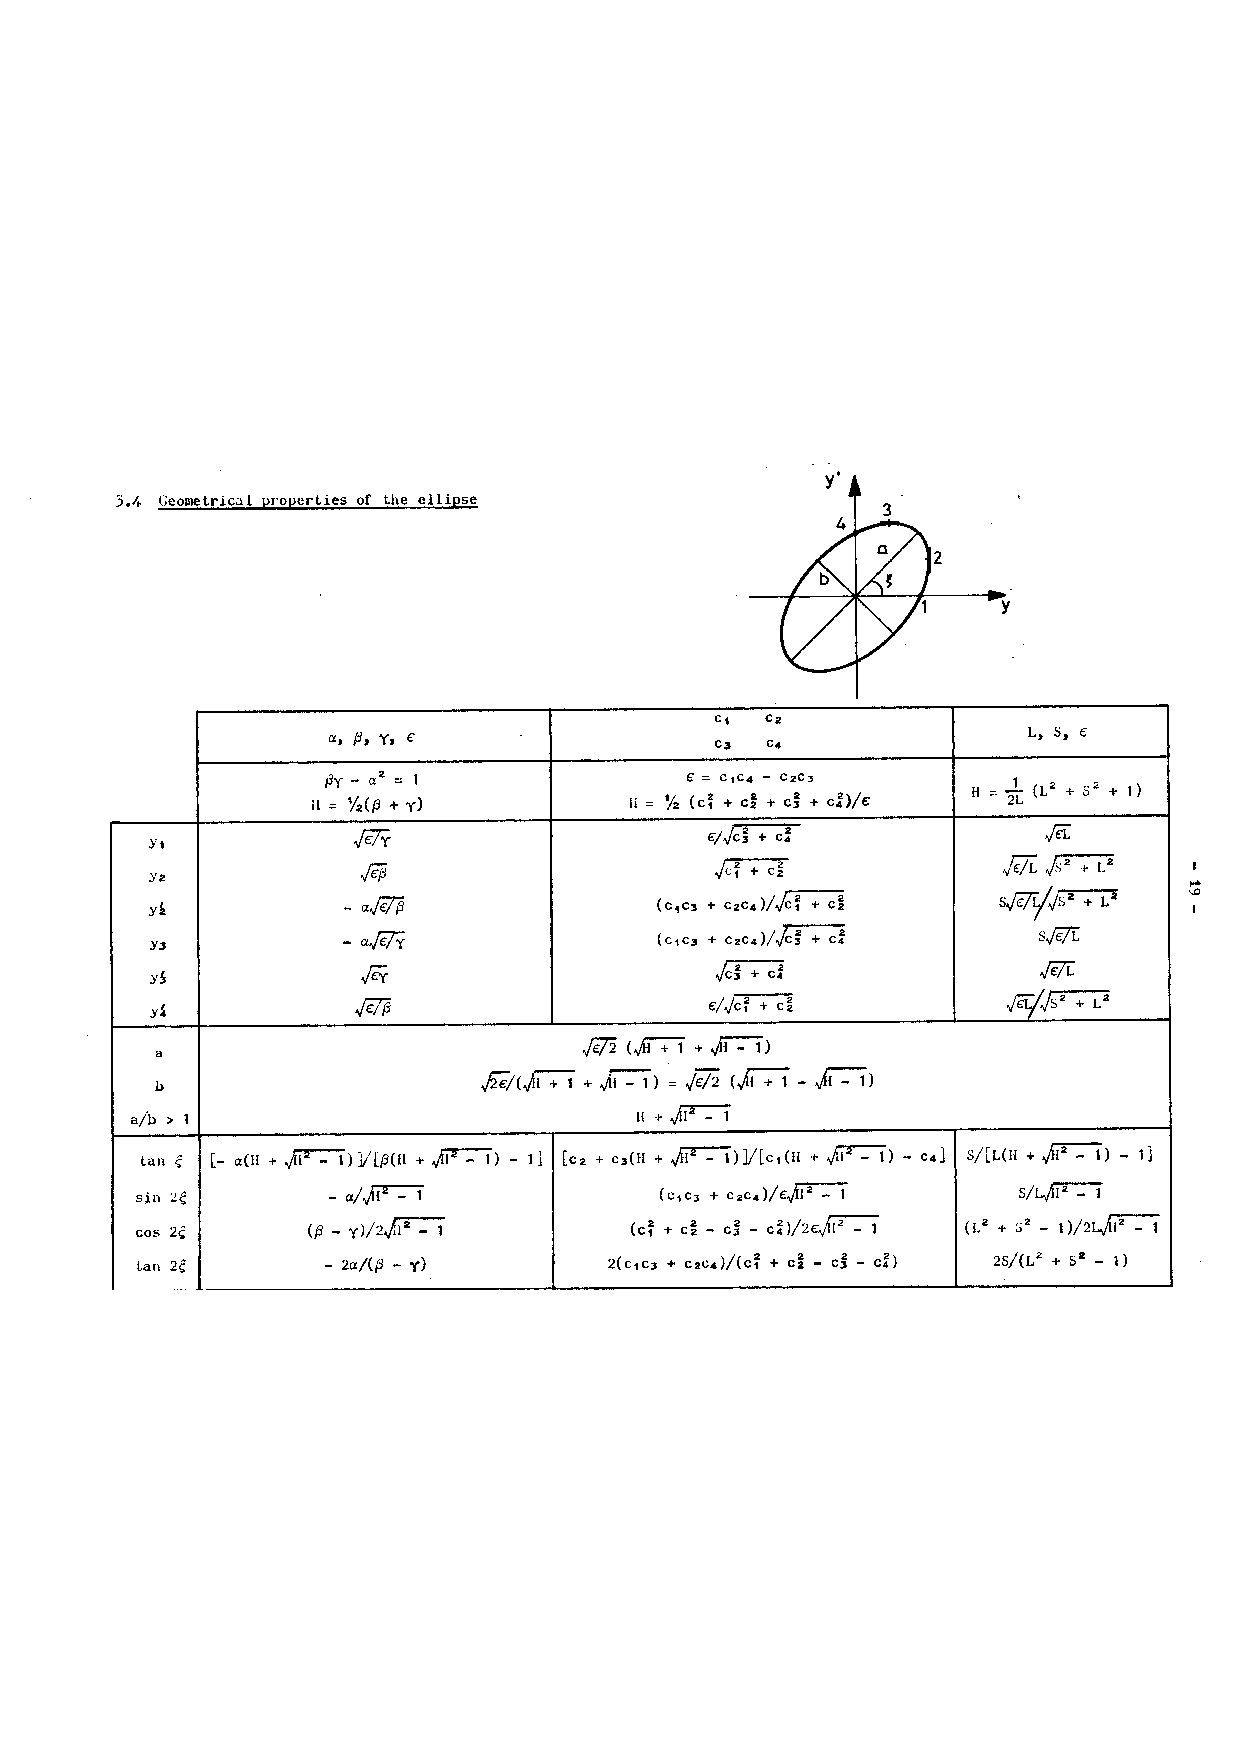
\includegraphics[width=15cm, trim={0.cm 7.6cm 0.cm 8.cm}, clip]{ellipse.pdf}

\end{document}
